% doctor.tex
%
% Aetf <aetf@unlimitedcodeworks.xyz>
% Copyright 2016 Aetf <aetf@unlimitedcodeworks.xyz>
%
% multiple1902 <multiple1902@gmail.com>
% Copyright 2011~2012, multiple1902 (Weisi Dai)
%
% Project Home: https://github.com/Aetf/xjtuthesis
%
% It is strongly recommended that you read documentations located at
%   https://github.com/Aetf/xjtuthesis/wiki
% in advance of your compilation if you have not read them before.
%
% This work may be distributed and/or modified under the
% conditions of the LaTeX Project Public License, either version 1.3
% of this license or (at your option) any later version.
% The latest version of this license is in
%   http://www.latex-project.org/lppl.txt
% and version 1.3 or later is part of all distributions of LaTeX
% version 2005/12/01 or later.
%
% This work has the LPPL maintenance status `maintained'.
%
% The Current Maintainer of this work is Aetf.
%
\documentclass[
    doctor,
    %propfont, % whether to use property fonts
    %nofont, % remember to manally set the fonts
    pdflinks,
    %colorlinks,
    %compact,
    ]{xjtuthesis}

\graphicspath{{figures/}}

\begin{document}

    
% 标题,中文
\ctitle{基于神经网络模型的人体姿态估计}

% 作者,中文
\cauthor{杜涵文}

% 学科,中文,本科生不需要
\csubject{}

% 学院,专业,班级,中文,本科毕业论文需要
\ccollege{电信}   % TODO 电信 or 计算机
\cmajor{计算机科学与技术}
\cclass{计算机少71}

% 设计所在单位,中文,本科毕业论文需要
\corgnization{西安交通大学}

% 学号
\stunum{2150506076}

% 导师姓名,中文
\csupervisor{魏平}

% 关键词,中文。用全角分号「;」分割
% 研究生的应首先从《汉语主题词表》中摘选
\ckeywords{人体姿态识别;动作捕捉;卷积神经网络;残差网络}

% 提交日期,本科生不需要
\cproddate{\the\year 年\the\month 月}

% 论文类型,中文,本科生不需要
% 从理论研究、应用基础、应用研究、研究报告、软件开发、设计报告、案例分析、调研报告、其它中选择
\ctype{}

% 论文标题,英文
\etitle{Human Pose Estimation Based on Deep Learning}

% 作者姓名,英文
\eauthor{Du Hanwen}
%todo 名字可能有错

% 学科,英文,本科生不需要
\esubject{}

% 导师姓名,英文
\esupervisor{Wei Ping}

% 关键词,英文。用半角分号和一个半角空格「; 」分割
\ekeywords{Human pose estimation; Motion capture; Convolutional neural networks; Residual networks}

% 学科门类,英文
% 从Philosophy(哲学)、Economics(经济学)、Law(法学)、Education(教育学)、Arts(文学)、
%   Science(理学)、Engineering Science(工学)、Medicine(医学)、Management Science(管理学)中选择 
\ecate{}

% 提交日期,英文,本科生不需要
% 应当和 cproddate 保持一致
\eproddate{\monthname{\month}\ \the\year}

% 论文类型,英文,本科生不需要
% 从Theoretical Research(理论研究)、Application Fundamentals(应用基础)、Applied Research(应用研究)、
%   Research Report(研究报告)、Software Development(软件开发)、Design Report(设计报告)、
%   Case Study(案例分析)、Investigation Report(调研报告)、其它(Other)中选择
\etype{}

% 摘要,中文。段间空行
\cabstract{

计算机视觉为人类社会工业界的重要支柱技术之一。随着深度学习的广泛应用,计算机视觉中人体姿态估计(HPE, human pose estimation)任务被注入了新的活力。同时随着基于摄像头的计算机视觉解决方案的广泛铺开,人体姿态估计在人机交互、游戏、虚拟现实、视频监控、运动分析、医疗辅助等领域有着广泛的应用。本文基于单目摄像头的视频采集,利用深度神经网络,完成了视频序列中单人的人体姿态估计任务,并有效地利用提取出的动作制作了人体模型三维动画。

人体姿态估计有诸多子课题,本文的工作主要聚焦在了单目单人RBG视频的三维人体姿态上。本文的工作选取了三维人体姿态估计中经典的两步提升思路,先将视频或图像中的人体关节点进行识别,预测出较为准确的二维坐标,再在此二维坐标结果的基础上预测出关节点的三维坐标。

在二维人体姿态估计上,采用了ResNet结构加以反卷积层,生成高分辨率的热力图以预测二维坐标。在三维人体姿态估计上,采用了一维空洞卷积网络处理视频序列间的时序信息,最终生成人体关节点的三维坐标序列。

最终,本文将人体姿态估计的实际应用场景定位在了动作捕捉三维角色动画生成上。利用上述的网络模型,针对日常的单人视频,提取出姿态序列。将其转换为动作捕捉记录文件类型后,对人体模型进行动作绑定,进而制作生动流畅还原度较高的三维角色动画。

}

% 摘要,英文。段间空行
\eabstract{

Computer vision is one of the important pillar technologies of human society industry. With the wide application of deep learning, the task of human pose estimation (HPE) in computer vision field has been injected with new vitality. At the same time, with the wide spread of camera-based computer vision solutions, human pose estimation has a wide range of applications in human-computer interaction, games, virtual reality, video surveillance, motion analysis, medical assistance and other fields. In this thesis, based on the video collection of monocular camera, the deep neural network is used to complete the single human body pose estimation task in the video sequence, and the 3D animation of human body model is made effectively by using the extracted actions.

There are many subjects of body pose estimation, and the work of this thesis mainly focuses on the 3D body pose of monocular single-person RBG video.The work of this thesis selects the classical two-step lifting idea in 3D body pose estimation. First, the body nodes in the video or image are identified to predict the more accurate 2D coordinates, and then the 3D coordinates of the nodes are predicted on the basis of the 2D coordinate results.

ResNet and deconvolution layer are used to estimate the 2D pose. Heat map is generated to predict the 2D coordinates. In 3D human pose estimation, a one-dimensional void convolutional network is used to process the time sequence information between video sequences, and finally generates the 3D coordinate sequence of human body nodes.

Finally, the actual application scene of human pose estimation is positioned in motion capture 3D character animation. Using the above network model, pose sequence is extracted for daily single person video. After converting it into motion capture record file type, action rigging is carried out on the human model to produce vivid 3D character animation.


}


    \xjtuchead
    \xjtuehead
    \xjtucinfopage
    \xjtueinfopage
    \xjtutoc
    \xjtutoe
    \clearpage

    % denotation.tex
%
% Aetf <aetf@unlimitedcodeworks.xyz>
% Copyright 2016 Aetf <aetf@unlimitedcodeworks.xyz>
%
% multiple1902 <multiple1902@gmail.com>
% Copyright 2011~2012, multiple1902 (Weisi Dai)
%
% Project Home: https://github.com/Aetf/xjtuthesis
%
% It is strongly recommended that you read documentations located at
%   https://github.com/Aetf/xjtuthesis/wiki
% in advance of your compilation if you have not read them before.
%
% This work may be distributed and/or modified under the
% conditions of the LaTeX Project Public License, either version 1.3
% of this license or (at your option) any later version.
% The latest version of this license is in
%   http://www.latex-project.org/lppl.txt
% and version 1.3 or later is part of all distributions of LaTeX
% version 2005/12/01 or later.
%
% This work has the LPPL maintenance status `maintained'.
%
% The Current Maintainer of this work is Aetf.
%
\begin{denotation}

  \item[\xjtuthesis]    我能吞下玻璃而不伤身体噢
  \item[Linux]          李氏操作系统
  \item[Windows]        温氏操作系统

\end{denotation}


    \xjtucontent

        
\chapter{绪论}
\echapter{Preface}

视觉在是人类的重要感官之一,也是人类获取信息效率最高的感官,是人类认识和理解外界的重要途经,计算机视觉也相应成为了人类社会工业界的重要支柱技术之一。随着深度学习的广泛应用,计算机视觉在近年有了蓬勃的发展,人体姿态估计(HPE, Human Pose Estimation)任务也被注入了新的活力,有了越来越多的科研成果。同时随着基于摄像头的计算机视觉解决方案的广泛铺开,人体姿态估计也逐渐贴合了越来越多的实际场景,在人机交互、游戏、虚拟现实、视频监控、运动分析、医疗辅助等领域有着广泛的应用,是计算机视觉领域的热门研究课题。本文基于单目摄像头的视频采集,利用深度神经网络,完成了视频序列中单人的人体姿态估计任务,并有效地利用提取出的动作制作了人体模型三维动画。



\section{应用背景与意义}


人体姿态估计在实际应用中,为视频监控、行为分析、自动驾驶、虚拟现实、人机交互(HCI, Humancomputer interaction)、医疗辅助、游戏、电影和动画等多种场景提供了丰富的人体几何和运动信息。

例如在视频监控中,利用人体识别与人体姿态识别,可以实时监控楼宇、工地、社区等场所的高风险区域,发现攀高等危险行为时及时告警提醒,避免异常攀高导致安全事故;或对公共场所中人员突然奔跑或突然的人员聚集等情况进行检测和预判,助于安防疏导。在行为分析方面,如图\reg{fig:f1}所示,人体姿态识别可以辅助体育运动和训练中,对运动员或训练者的动作进行分析,分析其运动的习惯,辅助教练对不规范动作进行纠正等。在自动驾驶的研发中,需要对车辆行驶的路况进行分析和预测,此时需要对行人的朝向,姿态进行分析,进而预测可能的下一步行为,帮助车辆依此进行行驶决策。在人机交互中,如图\reg{fig:f2}所示,可以利用对人体动作的识别研发远程交互式体感游戏。

\begin{figure}[h!]
  \centering
  \subfloat[人体姿态估计辅助体育运动分析] {
      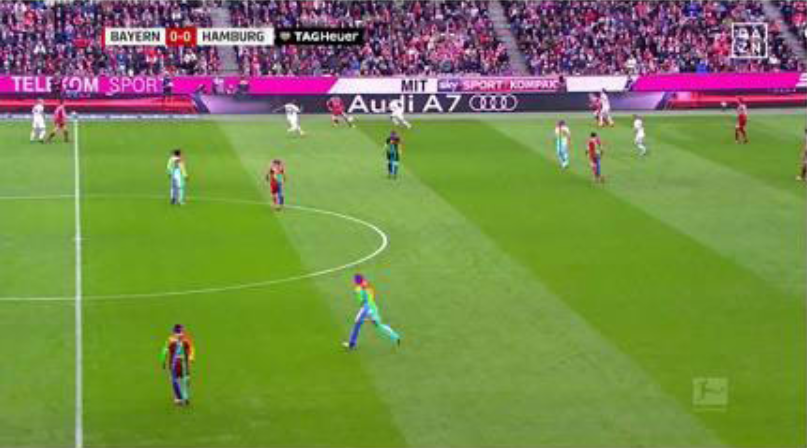
\includegraphics[width=6.67cm]{figures/1.png}
      \label{fig:f1}}
  \subfloat[基于人体姿态估计的体感游戏] {
      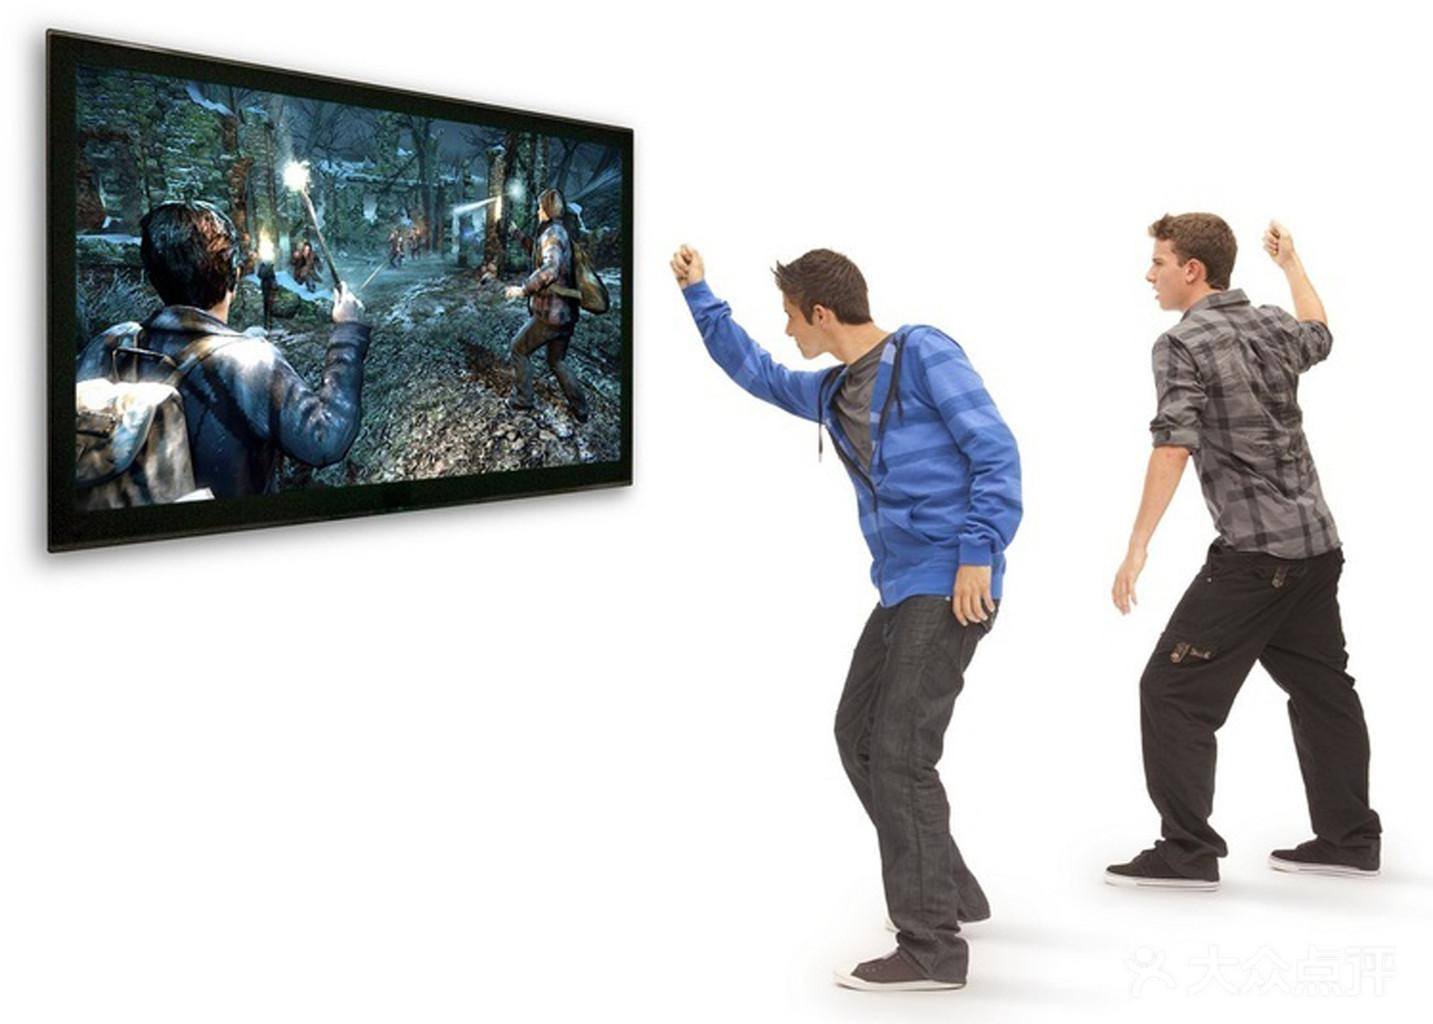
\includegraphics[width=6.67cm]{figures/2.png}
      \label{fig:f2}}
  \caption{人体姿态估计实际应用}
\end{figure}

人体姿态识别在近年来成为了人类社会各类产业中辅助生产的重要技术之一,本文的工作则将人体姿态识别应用在了影视动画创作领域,利用对视频中人体动作的分析,自动化生成具有相应动作的三维角色动画。

动作捕捉(MoCap, Motion Caption)是记录运动并在数字角色模型上创建运动的过程。动作捕捉可用于各种应用场景,例如运动,医疗应用,人体工程学,娱乐和机器人技术,以及三维角色动画,预可视化以及虚拟电影制作。更为具体地,当动作捕捉应用于游戏开发和电影制作中时,则主要指记录演员动作,来制作动画等具有视觉效果的媒体内容。

\begin{figure}[h]
	\centering
	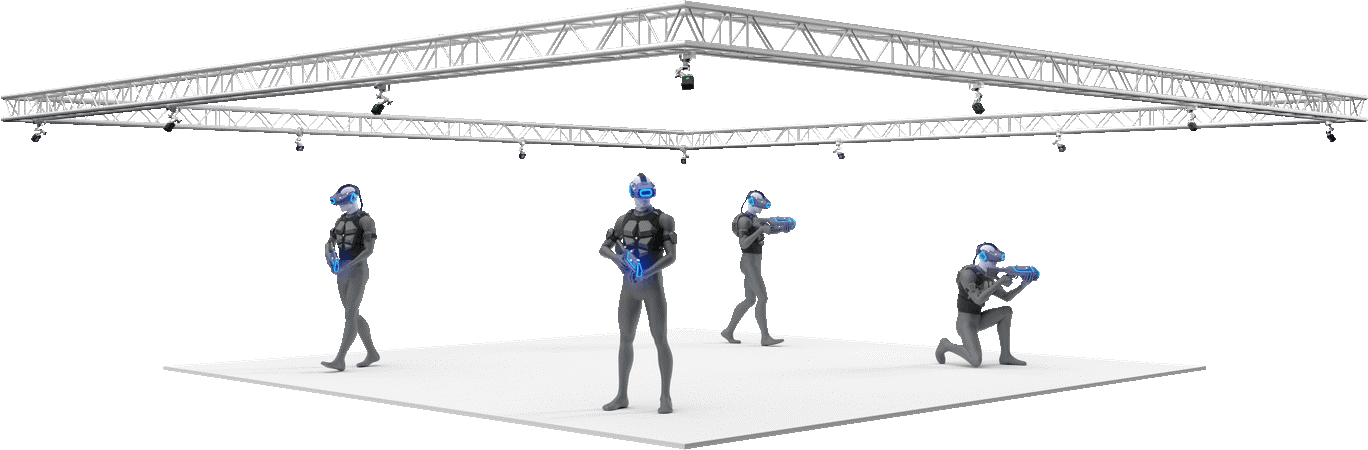
\includegraphics[scale=0.4]{figures/3.png}
	\caption{动作捕捉场地}
	\label{fig:f3}
\end{figure}

而这其中的主要动作捕捉技术主要依赖于硬件设备,从硬件设备的采集数据的原理上来说可以分为光学式、惯性式等。而除了一般动作捕捉系统中的穿戴式设备外、感应摄像头、符合光线要求的场地场所、相应软件以及基础的服务等对专业性的要求极高,价格不菲。根据相关调研报告,全球动作捕捉市场在2018年达到了1.632亿美元,并且预计到2026年,可以增长至2.617亿美元。同时预测复合年增长率在2019-2026年内为8.13%。

由于动作捕捉的价格昂贵,市场需求大,对动捕质量的要求随着动画产业的发展也在不断地增加。同时随着三维人体姿态估计的效果逐步提升,基于RGB摄像视频的动作捕捉成为了降低动画生成门槛的新的解决方案。



\section{课题主要任务}{}

人体姿态估计指在从图像或视频中,对任务目标的姿态进行识别和估计。

输入数据一般为采集的RGB图像或RGB-D图像,可以为单目单视角(Monocular)图像或使用多个摄像机针对相同的目标同一时刻的动作进行采集的多目多视角(Multi-view)图像,图像中可以包含一个人体目标或多个人体目标。

首先通过人体识别获得每个目标人体所在的区域或边框(bounding box),进一步通过热力图(heatmap)

对人体的各个关键点位置进行概览预测或直接回归出各关键点的坐标。可以通过对头部、颈部、髋部、膝盖等人体的重要关节点进行坐标预测来描述人体骨架,或通过估计出符合人体形状的蒙皮描述人体的姿态,例如图\reg{fig:f4}右侧蒙皮图像所示,SMPL模型(Skinned Multi-Person Linear (SMPL) Model),便利用具有10个维度的形状参数和描述24个关节点的姿态参数描述整个人体的蒙皮。

\begin{figure}[h]
	\centering
	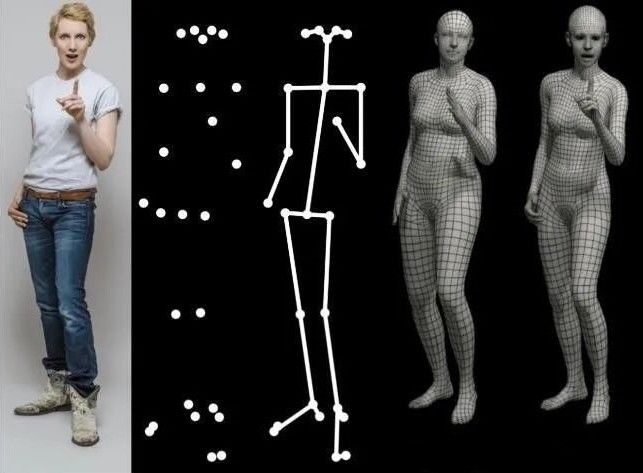
\includegraphics[scale=0.4]{figures/4.jpg}
	\caption{人体姿态描述模型}
	\label{fig:f4}
\end{figure}

此外,可以仅针对单帧图像进行估计,也可以在视频中,针对帧序列中的人体进行姿态序列的分析。在对帧序列进行姿态估计时,需要对同一个目标人物进行追踪,并利用时序模型来提取上下文信息,估计出准确连贯的姿态序列。

最为主要地,根据输出的数据维度,也即描述人体姿态关节点的坐标维度,可以划分为二维人体姿态估计与三维人体姿态估计两大部分。二维人体姿态估计的目标是定位图像中每个关键点的(x,y)坐标,而三维人体姿态估计的目标是推断三维空间中每个关键点的(x,y,z)坐标。

本文的工作主要集中在了对单目单人RGB视频中的目标进行姿态估计。基于此类数据的人体关节点坐标的恢复具有其独特的特征和挑战,其挑战主要在于三点:

其一,柔性体构型意味着复杂的相互依赖的关节和高自由度的肢体,这可能会导致出现自遮挡及其他罕见且复杂的姿态。

其二,是人体呈现的多样性,包括服装的多样及自身极为相似的部位。

其三,复杂的拍摄环境常导致前景的遮挡,加之多样的拍摄角度和画幅的不完整,导致目标与周围人的相似部位出现混淆。



\section{国内外研究现状}

\subsection{二维人体姿态估计}{}

早期的二维人体姿态估计融入了许多特征的构建,比如描述运动信息的梯度方向直方图(HOG, Histogram of Oriented Gradient)和小边特征(Edgelet)
等,但这些方法在实践中并不具备精确估计的能力。随着深度神经网络的发展,深度学习方法则更能够从元数据重提取出更充分的特征,产生了优异的结果,并在很大程度上超过了传统方法。基于方法分类的二维人体姿态估计任务如图\reg{fig:f5}。

\begin{figure}[h]
	\centering
	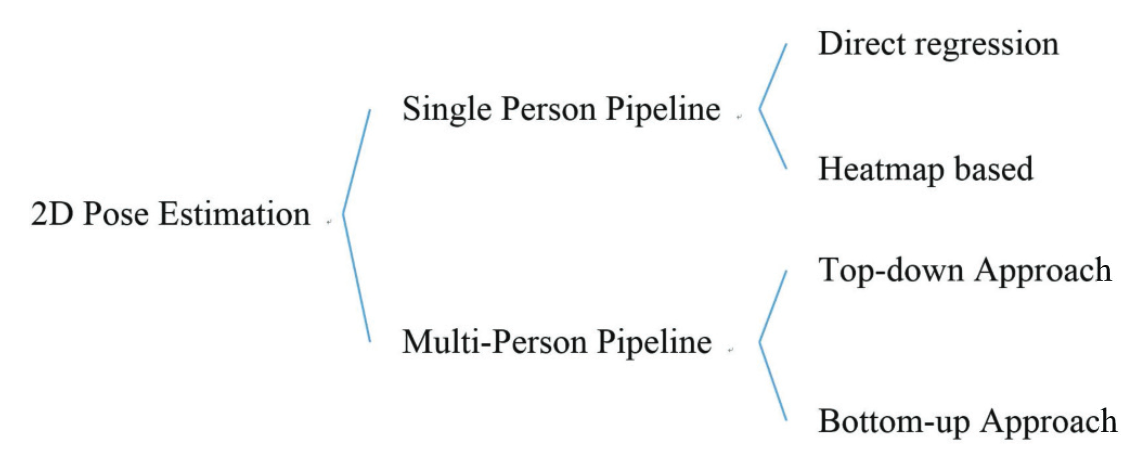
\includegraphics[scale=0.4]{figures/5.png}
	\caption{二维人体姿态估计分类}
	\label{fig:f5}
\end{figure}

单人姿态估计从预测关键点的方法上主要分为直接回归方法与热力图方法两类。前者利用输出特征映射直接回归关键点,如facebook于2018年搭建的DensePose。后者则首先生成热图(heatmap),用其中的像素值表示关键点在该位置存在的概率,并根据热图预测关键点,如2016年的Hourglass。

而多人姿态估计的整体思路主要分为两类。第一种为自顶向下的方法,指的是首先从全图的范围上进行人体检测,然后切入到每个目标人体的范围,进行单人关键点估计,如2016年提出的AlphaPose。自底向上的方法的第一步则是定位图像中的所有关节点,第二步是将关节点向上分组为人体,2016年提出利局部关联域(PAF, Part Affinity Field)方法进行关键点组装的OpenPose。

\subsection{三维人体姿态估计}{}
三维人体姿态估计相对于二维人体姿态估计具有更多难点,其一是单目图像及视频信息本身具有的歧义性,即一个二维的姿态投影可以对应多种三维的姿态。其二是需要利用昂贵的设备和严苛的环境条件进行三维姿态数据集的采集较为困难,故而对网络的泛化性要求也更为严格。

\begin{figure}[h]
	\centering
	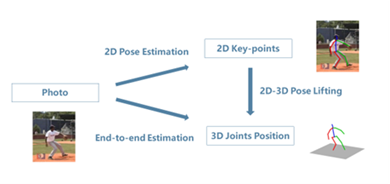
\includegraphics[scale=0.4]{figures/6.png}
	\caption{三维人体姿态估计两大思路}
	\label{fig:f6}
\end{figure}

如图\reg{fig:f6}所示,基于深度学习的三维人体姿态估计方法可主要分为两大思路。第一种思路为两步式,先从图像中提取出二维关节点坐标,再将其从二维提升到三维坐标,如Facebook AI于2018年提出的VideoPose三维模型。第二种思路为端到端式,从视频和图像中直接回归出三维坐标,如Li等于2014年利用卷积神经网络搭建的包括关节检测与坐标回归两支路模型。此外,还有工作选择融合式模型,在两步式的第二步估计过程中仍然融入源数据。

\subsection{视频动作捕捉}{}
无硬件设备需求的视频人体动作捕捉解决方案提供商在近几年,于国内外如雨后春笋般崛起并在持续地发展。

如国内云舶提供的对单人视频进行捕捉的小K动捕,对人物的脚-地接触进行了优化,使其接触稳定,无垂直的浮动。此外,美国DeepMotion也提供了包含单人动作捕捉以及人物追踪等多种视频解决方案。同时,Ridical也提供了粒度细至手指关节的实时视频动作捕捉API。

\begin{figure}[h]
	\centering
	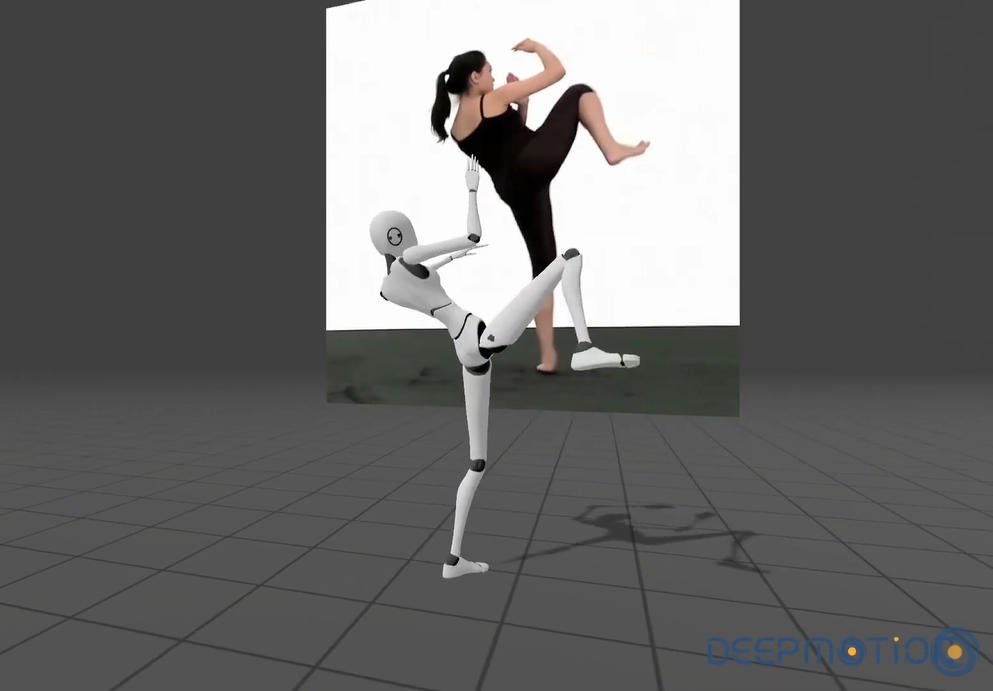
\includegraphics[scale=0.4]{figures/7.png}
	\caption{DeepMotion视频动作捕捉}
	\label{fig:f7}
\end{figure}



\section{本文主要工作内容}


\subsection{本文工作}{}
针对人体姿态估计任务,本文的工作主要聚焦到了基于深度神经网络模型,对日常场景中,单目RGB摄像头采集的单人动作视频进行姿态估计,并利用估计出的人物动作制作三维角色动画。整体流程首先输入单人视频,利用残差网络搭建二维关节点估计模型,并利用一维空洞卷积提取视频中的时序信息,将二维关节点坐标提升为三维坐标,最后将三维坐标转换为描述动作文件的人体骨架欧拉角,进行三维角色绑定。

\subsection{论文结构安排}{}
本文共包含六个章节,各章节的具体内容概括如下。

第一章:绪论。在绪论中,首先介绍了人体姿态估计课题的研究意义以及在各实际领域的应用价值,尤其是在动作捕捉领域,具有旷阔的市场和可期的前景。接着介绍了人体姿态估计的任务的具体目标及当前工作的研究现状。最后对本文的主要工作进行了简要的概括 ,并对本文的章节安排进行了介绍。

第二章:人体姿态识别相关基础。在第二章中,针对计算机视觉尤其是人体姿态估计中常用到的经典的深度学习模型及方法进行了介绍,包括卷积神经网络、残差网络等,它们构成了第三章及第四章模型的基础架构。同时介绍了人体姿态描述模型与动作捕捉相关设备与数据文件。

第三章:基于反卷积神经网络的二维人体姿态估计。本章重点说明了用于二维人体姿态估计的模型,一个相对于之前的Hourglass和CPN结构都更为简单明了的网络结构。模型利用热力图对人体关节进行二维坐标的预测,并在网络中利用反卷积进行上采样,用以得到高分辨率的特征图。

第四章:基于空洞卷积神经网络的三维人体姿态序列估计。本章首先针对三维人体姿态估计任务的主要问题进行了分析,并采用了二步提升法,同时利用卷积神经网络处理视频中的时序信息,进行三维人体姿态的估计。

第五章:视频动作捕捉动画生成。在本章中,利用第三章及第四章的网络模型所预测出的人体姿态,对人物角色模型进行动画生成。搭建了人体骨骼模型,将关节点坐标转换为了动作描述文件bvh所需的欧拉角。并在MotionBuilder软件中对人物模型进行了动作绑定,制作出了还原度极高且稳定的三维动画。

第六章:总结与展望。本章归纳和总结了本文针对人体姿态估计任务所做的工作,以及针对视频动作捕捉进行的工程搭建。对人体姿态估计的后续研究方向以及视频动作捕捉的未来进行了更深层次的探讨和展望。





        % float.tex
%
% Aetf <aetf@unlimitedcodeworks.xyz>
% Copyright 2016 Aetf <aetf@unlimitedcodeworks.xyz>
%
% multiple1902 <multiple1902@gmail.com>
% Copyright 2011~2012, multiple1902 (Weisi Dai)
%
% Project Home: https://github.com/Aetf/xjtuthesis
%
% It is strongly recommended that you read documentations located at
%   https://github.com/Aetf/xjtuthesis/wiki
% in advance of your compilation if you have not read them before.
%
% This work may be distributed and/or modified under the
% conditions of the LaTeX Project Public License, either version 1.3
% of this license or (at your option) any later version.
% The latest version of this license is in
%   http://www.latex-project.org/lppl.txt
% and version 1.3 or later is part of all distributions of LaTeX
% version 2005/12/01 or later.
%
% This work has the LPPL maintenance status `maintained'.
%
% The Current Maintainer of this work is Aetf.
%
\chapter{浮动格式}

    金溪民方仲永,世隶耕。仲永生五年,未尝识书具,忽啼求之。父异焉,借旁近与之,即书诗四句,并自为其名。其诗以养父母、收族为意,传一乡秀才观之。自是指物作诗立就,其文理皆有可观者。邑人奇之,稍稍宾客其父,或以钱币乞之。父利其然也,日扳仲永环谒于邑人,不使学。

    余闻之也久。明道中,从先人还家,于舅家见之,十二三矣。令作诗,不能称前时之闻。又七年,还自扬州,复到舅家问焉。曰:“泯然众人矣。”

    王子曰:仲永之通悟,受之天也。其受之天也,贤于才人远矣。卒之为众人,则其受于人者不至也。彼其受之天也,如此其贤也,不受之人,且为众人;今夫不受之天,固众人,又不受之人,得为众人而已耶?

    \section{图片}

        \begin{figure}[h!]
          \centering
          
\includegraphics[width=6.67cm]{XJTU.pdf}
          \caption{西安交通大学}
          \label{fig:xjtu}
        \end{figure}

        \begin{figure}[h!]
          \begin{minipage}{0.45\textwidth}
              \centering
              
\includegraphics[width=6.67cm]{XJTU.pdf}
              \caption{西安交通大学}
              \label{fig:xjtu-left}
          \end{minipage}
          \begin{minipage}{0.45\textwidth}
              \centering
              
\includegraphics[width=6.67cm]{XJTU.pdf}
              \caption{西安交通大学}
              \label{fig:xjtu-right}
          \end{minipage}
        \end{figure}
          
        \begin{figure}[h!]
          \centering
          \subfloat[果毅力行]{
              
\includegraphics[width=6.67cm]{XJTU.pdf}
              \label{fig:xjtu-sub-left}}
          \subfloat[忠恕任事]{
              
\includegraphics[width=6.67cm]{XJTU.pdf}
              \label{fig:xjtu-sub-right}}
          \caption{子图}
        \end{figure}
          

    \section{表格}

        \begin{table}[h!]
          \centering
          \caption{一个简单的表格}
          \label{tab:simple}
          \wuhao
          \begin{tabularx}{\linewidth}{XXXXX} \toprule 
                & 一月 & 二月 & 三月 & 合计 \\ \midrule
           东部 &    7 &    7 &    5 &   19 \\ 
           西部 &    6 &    4 &    7 &   17 \\ 
           南部 &    8 &    7 &    9 &   24 \\ 
       \bf 合计 &   21 &   18 &   21 &   60 \\ \bottomrule
          \end{tabularx}
        \end{table}


        \begin{table}[h!]
          %\begin{minipage}{\textwidth}
          \begin{threeparttable}[h]
            \centering
            \caption{包含脚注的表格}
            \label{tab:with-footnote}
            \wuhao
            \begin{tabularx}{\linewidth}{XXXXX} \toprule 
                  & 一月 & 二月 & 三月 & 合计 \\ \midrule
                  东部 &    7\tnote{1}
                                &    7 &    5 &   19 \\ 
             西部 &    6 &    4 &    7 &   17 \\ 
             南部 &    8 &    7 &    9 &   24 \\ 
             \bf 合计\tnote{2}
                  &   21 &   18 &   21 &   60 \\ \bottomrule
            \end{tabularx}
          %\end{minipage}
          \begin{tablenotes}
          \item[1] 数据来自Word 97.
          \item[2] Computed by \textsl{Mathematica} 8.
          \end{tablenotes}
          \end{threeparttable}
        \end{table}

        \begin{table}[h!]
          \centering
          \caption{稍微复杂一点的表格}
          \label{tab:complex}
          \wuhao
          \begin{tabularx}{\linewidth}{XXXXX} \toprule 
                & \multicolumn{3}{c}{这是一句废话} &  \\ \cmidrule{2-4}
                & 一月 & 二月 & 三月 & 合计 \\ \midrule
           东部 &    7 &    7 &    5 &   19 \\ 
           西部 &    6 &    4 &    7 &   17 \\ 
           南部 &    8 &    7 &    9 &   24 \\ 
       \bf 合计 &   21 &   18 &   21 &   60 \\ \bottomrule
          \end{tabularx}
        \end{table}

        我制作了一个简单的表格(表\ref{tab:simple})。



        % formulae.tex
%
% Aetf <aetf@unlimitedcodeworks.xyz>
% Copyright 2016 Aetf <aetf@unlimitedcodeworks.xyz>
%
% multiple1902 <multiple1902@gmail.com>
% Copyright 2011~2012, multiple1902 (Weisi Dai)
%
% Project Home: https://github.com/Aetf/xjtuthesis
%
% It is strongly recommended that you read documentations located at
%   https://github.com/Aetf/xjtuthesis/wiki
% in advance of your compilation if you have not read them before.
%
% This work may be distributed and/or modified under the
% conditions of the LaTeX Project Public License, either version 1.3
% of this license or (at your option) any later version.
% The latest version of this license is in
%   http://www.latex-project.org/lppl.txt
% and version 1.3 or later is part of all distributions of LaTeX
% version 2005/12/01 or later.
%
% This work has the LPPL maintenance status `maintained'.
%
% The Current Maintainer of this work is Aetf.
%
\chapter{公式环境}

    \begin{axiom}
        \rm 两点间直线段距离最短。  
        \begin{align}
            x&\equiv y+1\pmod{m^2}\\
            x&\equiv y+1\mod{m^2}\\
            x&\equiv y+1\pod{m^2}
        \end{align}
    \end{axiom}

    \begin{remark}
    \rm 对齐的公式示例,它还同时演示了标号。
    \begin{align}
    \begin{split} 
    \varphi(x,z)
    &=z-\gamma_{10}x-\gamma_{mn}x^mz^n\\
    &=z-Mr^{-1}x-Mr^{-(m+n)}x^mz^n
    \end{split} \notag \\
    \noindent\zeta^1&=(\xi^1)^2,\\
    \zeta^1 &=\xi^0\xi^1,\\
    \zeta^2 &=(\xi^1)^2,
    \end{align}
    \end{remark}

    \begin{theorem}
      \rm 对于直角三角形$ABC$, 若$a<c$且$b<c$, 则有
        \begin{equation}
          a^2+b^2=c^2
        \end{equation}
    \end{theorem}


    \begin{exercise}
          \rm 请列出温家宝的所有影视作品。
    \end{exercise}
        
    贝叶斯公式如式~(\ref{equ:chap1:bayes}),其中 $p(y|\mathbf{x})$ 为后验;
    $p(\mathbf{x})$ 为先验;分母 $p(\mathbf{x})$ 为归一化因子。
    \begin{equation}
        \label{equ:chap1:bayes}
        p(y|\mathbf{x}) = \frac{p(\mathbf{x},y)}{p(\mathbf{x})}=
        \frac{p(\mathbf{x}|y)p(y)}{p(\mathbf{x})} 
    \end{equation}


        % monet.tex
%
% Aetf <aetf@unlimitedcodeworks.xyz>
% Copyright 2016 Aetf <aetf@unlimitedcodeworks.xyz>
%
% multiple1902 <multiple1902@gmail.com>
% Copyright 2011~2012, multiple1902 (Weisi Dai)
%
% Project Home: https://github.com/Aetf/xjtuthesis
%
% It is strongly recommended that you read documentations located at
%   https://github.com/Aetf/xjtuthesis/wiki
% in advance of your compilation if you have not read them before.
%
% This work may be distributed and/or modified under the
% conditions of the LaTeX Project Public License, either version 1.3
% of this license or (at your option) any later version.
% The latest version of this license is in
%   http://www.latex-project.org/lppl.txt
% and version 1.3 or later is part of all distributions of LaTeX
% version 2005/12/01 or later.
%
% This work has the LPPL maintenance status `maintained'.
%
% The Current Maintainer of this work is Aetf.
%
% Almost all text in this file are taken from Chinese Wikipedia at
%   https://zh.wikipedia.org/zh/克洛德·莫奈
% or 
%   https://zh.wikipedia.org/wiki/%E5%85%8B%E6%B4%9B%E5%BE%B7%C2%B7%E8%8E%AB%E5%A5%88
% and are released under Creative Commons Attribution-Share Alike License 3.0
% which can be found at 
%   https://en.wikipedia.org/wiki/Wikipedia:Text_of_Creative_Commons_Attribution-ShareAlike_3.0_Unported_License
%
\chapter{克洛德·莫奈}
\echapter{Claude Monet}

\begin{quotation}
    编者注:本章内容取自「维基百科,自由的百科全书」,并以创作共用「署名-相同方式共享」授权重新发布。\xjtuthesis 第一版的开发代号为~Monet。
\end{quotation}

    克洛德·莫奈\footnote{法语:Claude Monet,1840年11月14日 --- 1926年12月5日}(图\ref{fig:claude-monet}),法国画家,印象派代表人物和创始人之一。印象出自其代表作《印象·日出》的标题。

    \begin{figure}[h!]
      \centering
      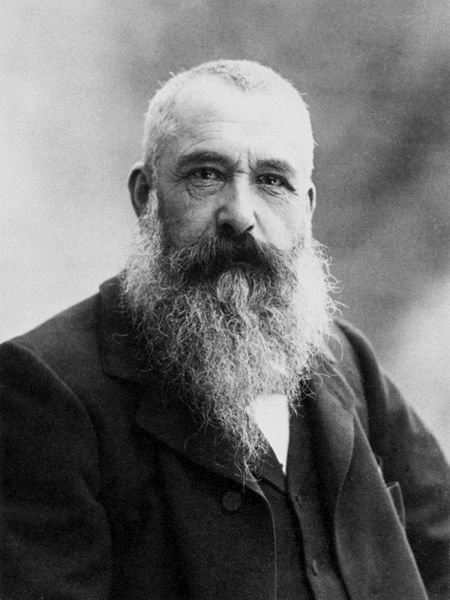
\includegraphics[width=6.67cm]{450px-Claude_Monet_1899_Nadar_crop.jpg}
      \caption{Claude Monet (公有领域)}
      \label{fig:claude-monet}
    \end{figure}

    莫奈是法国最重要的画家之一,印象派的理论和实践大部份都有他的推广。莫奈擅长光与影的实验与表现技法。他最重要的风格是改变了阴影和轮廓线的画法,在莫奈的画作中看不到非常明确的阴影,也看不到突显或平涂式的轮廓线。除此之外,莫奈对于色彩的运用相当细腻,他用许多相同主题的画作来实验色彩与光完美的表达。莫奈曾长期探索光色与空气的表现效果,常常在不同的时间和光线下,对同一对象作多幅的描绘,从自然的光色变幻中抒发瞬间的感觉。

    \section{早年生涯}
    \esection{Early Years}

        莫奈1840年11月14日出生于法国巴黎45街拉菲特第九郡,是阿道夫和路易斯的第二个儿子。他的父母都是第二代的巴黎人。1841年5月20日,他在当地的巴黎圣母院教区教堂受洗。在全家搬到了在诺曼底、位于塞纳河口北岸的勒阿弗尔\footnote{Le Havre}。他的父亲希望他继承家里的杂货店,但莫奈则想成为一个艺术家。他的母亲是一名歌手。

        1851年4月1日起,莫奈进入勒阿弗尔艺术中学。他的木炭漫画开价十到二十法郎,因此为当地人熟知。莫奈跟从雅克-弗兰柯伊斯·奥查德学习了最初的绘画课程,而后者是雅克-路易·大卫。在诺曼底的海滩上,他遇到了艺术家欧仁·布丹\footnote{Eugene Boudin},他后来成了莫奈的良师益友并教授他学会画油画。布丹教了莫奈绘画上的「空气」技法。

        1857年1月28日,他的母亲去世了。因此他从16岁起,离开学校,和丧偶无子女的姨妈玛丽-让娜·列卡德\footnote{Marie-Jeanne Lecadre}居住。

    \section{在巴黎}
    \esection{In Paris}

        当莫奈来到巴黎卢浮宫,他亲眼看到许多画家在模仿著名艺术家的作品。于是,随身携带着颜料和工具的他便坐在一扇窗户旁开始画他所看到的东西。莫奈在法国居住了数年,并与其他年轻画家会面。其中爱德华·马奈成为了他的好朋友,并且也是印象派画家。

        \begin{figure}[h!]
          \centering
          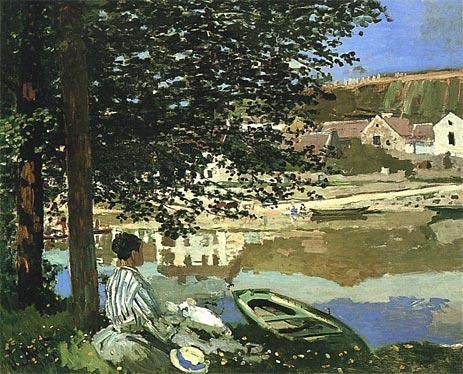
\includegraphics[width=6.67cm]{Claude_Monet_River_Scene_at_Bennecourt_Seine.jpg}
          \caption{\textit{On the Bank of the Seine, Bennecourt} (公有领域)}
          \label{fig:on-the-bank-of-the-seine}
        \end{figure}

        莫奈在阿尔及利亚当了两年兵\footnote{1860年 --- 1862年},在他服役七年的合同到期之前,因为伤寒,莫奈的姑妈Lecadre夫人将他从部队解脱出来,让他去完成大学的艺术课程。这可能是在他认识的荷兰画家Johan~Barthold~Jongkind的干预下完成的。

        因为大学的传统艺术教育让他觉醒,1862年莫奈在巴黎加入了夏尔·格莱尔\footnote{Charles Gleyre}画室。在那里他结认了皮耶-奥古斯特·雷诺阿、弗雷德里克·巴齐耶\footnote{Frederic Bazille}以及阿尔弗雷德·西斯莉\footnote{Alfred Sisley}。他们共同创造了一种新的艺术手法,即在户外和自然光线下用浓厚的油彩作画,后来被称为印象派。

        1866年,他以卡米耶·东西厄\footnote{Camille Doncieux}为模特创作了《绿衣女人》\footnote{\textit{The Woman in the Green Dress}}。这件作品使他受到承认。卡米耶也是他次年作品《花园中的女人》中的模特,还出现在他1868年在塞纳河岸上绘制的《塞纳河岸》中。不久之后,卡米耶即怀孕并生下了他们的第一个孩子让\footnote{Jean}。

    \section{普法战争,印象派,阿尔}
    \esection{Franco-Prussian War, Impressionism, and Argenteuil}

        在普法战争\footnote{Franco-Prussian War,1870年 --- 1871年}期间,莫奈于1870年9月来到英国避难。在那里他学习约翰·康斯太布尔和J·M·W·透纳\footnote{J.M.W.Turner}的作品。他们的作品激发了莫奈对色彩研究方面的创新。1871年春天,皇家艺术学院拒绝将莫奈的作品列入展览。

        1871年,他离开伦敦来到荷兰赞丹。在那里他创作了25幅作品,并且导致警察怀疑他在进行革命活动。他还首次游览了附近的阿姆斯特丹。1871年的10月或11月,他回到了法国。直到1878年,他基本都居住在法国阿尔,巴黎附近塞纳河右岸上的一个小村庄,那里也是受到巴黎人欢迎的郊游目的地。1874年,他短暂地返回了荷兰。

        \begin{figure}[h!]
          \centering
          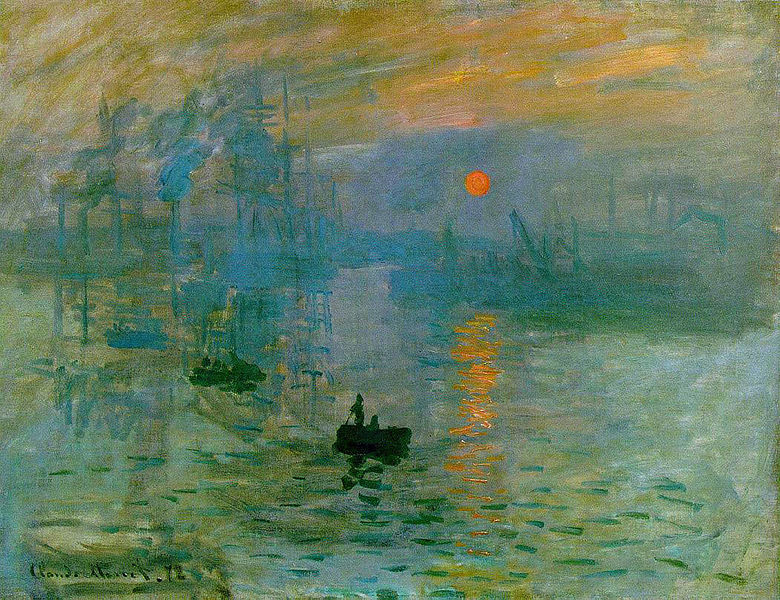
\includegraphics[width=6.67cm]{780px-Claude_Monet_Impression_soleil_levant_1872.jpg}
          \caption{印象·日出(公有领域)}
          \label{fig:impression-soleil-levant}
        \end{figure}
        
        1872年,莫奈以勒阿弗尔的一处风景为背景创作了《印象·日出》\footnote{\textit{Impression, soleil levant}}(图\ref{fig:impression-soleil-levant})。它在1874年第一次印象派画家展上亮相,如今它陈列在巴黎马蒙丹·莫奈美术馆\footnote{Muse Marmottan-Monet}。从这幅画的题目中,艺术评论家路易·勒鲁瓦提出了「印象派」的说法。莫奈有两幅关于林荫大道的画作,一副现在在莫斯科的普希金博物馆中,另一幅在堪萨斯城的纳尔逊-阿特金斯艺术博物馆中。人们从来都不清楚到底哪幅才是1874年展览中展出的,尽管近来人们倾向于认为是在莫斯科的那幅。
        1870年,莫奈与东西厄结婚。1871年,他们搬进了塞纳河\footnote{Seine River}边阿让特伊\footnote{Argenteuil}的一幢房子。正是在这个时期,莫奈创作了大量的作品。1876年,莫奈夫人生病了。1878年3月17日,他们有了另一个儿子,米歇尔\footnote{Michael}。1879年,莫奈夫人死于肺结核。

    \section{后来的日子}
    \esection{Later life}
        
        卡米尔去世后的数个月,伤心欲绝的莫奈为了不再陷入贫困而认真创作了一些19世纪最棒的绘画。19世纪80年代初,他绘制了几组风景和海景作为他在法国乡村生活的记录。这些记录演变成了他的系列画作。
        
        1878年莫奈一家暂时搬到Ernest~Hosched\footnote{1837年 --- 1891年}的房子中居住。他是一个富裕的百货商店老板,并且也是艺术赞助人。那个夏天,这两个家庭分享了在Vtheuil的这套房子。在那之后Ernest~Hosched破产了,并于1878年前往比利时。1879年,东西厄逝世后,莫奈依然居住在那里。Alice~Hoschede决定帮助莫奈抚养他的两个孩子,并带去巴黎,和她自己的六个孩子在一起。1880年他们从巴黎回来了。1881年,他们搬到了普瓦西\footnote{Poissy},但莫奈不喜欢那里。1883年4月,他们搬到了上诺曼底大区厄尔省的Giverny。他种植了一个大花园并在那里完成了他余生的绘画创作。莫奈和Alice~Hoschede在1892年结婚。
    
    \section{在吉维尼}
    \esection{Giverny}
    
        1883年5月初,莫奈和他的家族从本地的一个田主手中租下了一个房子。这个房子座落在Vernon和吉维尼的Gasny。房子中有一个谷仓被用作画室,但也是果园和小花园。房子离本地的学校很近,周围的景观给莫奈的作品提供了很多灵感。随着一家在此劳作,修耆院子,莫奈的作品也被经销商保罗·杜兰德-鲁埃尔越卖越多,他的命运得到了改变。直到1890年11月,莫奈已经买得起他的房子和周边建筑了。十九世纪90年代,莫奈创建了一个温室和他的第二个工作室,那是一个包含天窗的宽敞的建筑。
        
        在十九世纪八十年代和九十年代,莫奈开始了系列绘画创作,即在不同的光线和角度连续画同一个物体。他的第一个系列作品《鲁昂主教座堂》就是在不同的角度和一天中不同的时间来画。1895年,从20个不同角度对大教堂所作的画在迪朗德 --- 吕埃尔\footnote{Gurand-Ruel}画廊展出。此外,他的作品还有稻草堆系列、白杨系列、伦敦议会、塞纳河的早晨、睡莲系列。

        \begin{figure}[h!]
          \begin{minipage}{0.5\textwidth}
              \centering
              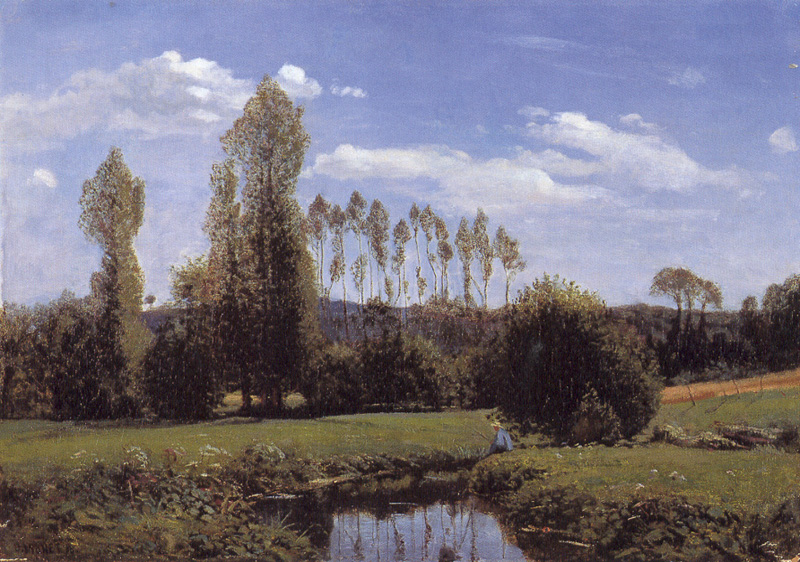
\includegraphics[width=6.67cm]{Monet-Claude_-_View_At_Rouelles_Le_Havre_1858.jpg}
              \caption{\textit{View At Rouelles, Le Havre} (公有领域)}
              \label{fig:view-at-rouelles-le-havre}
          \end{minipage}
          \begin{minipage}{0.5\textwidth}
              \centering
              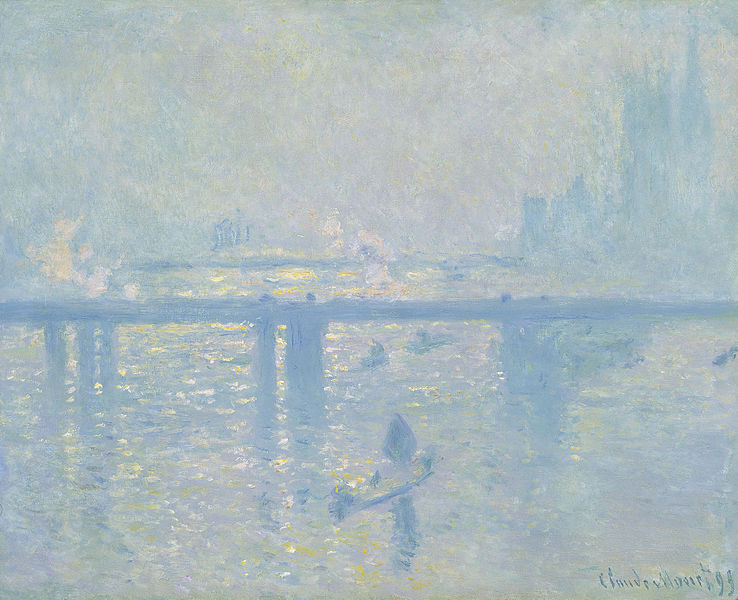
\includegraphics[width=6.67cm]{738px-Charing_Cross_Bridge_Monet.jpg}
              \caption{\textit{Charing Cross Bridge}  (公有领域)}
              \label{fig:charing-cross-bridge}
          \end{minipage}
        \end{figure}
        
        莫奈喜欢绘制受控状态下的自然:他在吉维尼的院子和里面的睡莲,还有桥。他还画了塞纳河的上上下下,产生了如塞纳河上的冰破裂了的画作。他每天给他的园丁写的指示中包含了精确的设计和种植布局,以及购买花卉和植物学书籍。与莫奈的财富增长伴随着的是他的花园的进化。甚至在他雇佣了7名园丁的时候,他依然保留了花园的建筑师。
        
        1883年至1908年间,莫奈在地中海画了许多风景画和海景画。在意大利威尼斯,他画了一系列重要的画作,在伦敦他绘制了两个重要的系列——议会系列和查林十字街大桥系列。他的第二个妻子,Alice,在1911年逝世。他特别喜欢的、娶了Alice的女儿布兰奇的大儿子,于1914年去世。妻子逝世后,布兰奇照顾和关心他。这段时间,莫奈身上出现了白内障的最初迹象。
        
        第一次世界大战期间,他年轻的儿子米歇尔参军,他的朋友、崇拜者乔治·克列孟梭领导法国。莫奈绘制了一系列垂柳树以表达对法国阵亡将士的敬意。1923年,莫奈接受了两次白内障手术,以减小他的画作受到白内障症状的影响:因为白内障影响了他的视力,画作整体偏红。也可能是这样:他在手术后可以看到某些正常人看不见的紫外线,这会影响到他观察到的颜色。在手术后,他甚至重新绘制了他的作品,其中的睡莲(图\ref{fig:water-lilies})更蓝了。


        \begin{figure}[h!]
          \centering
          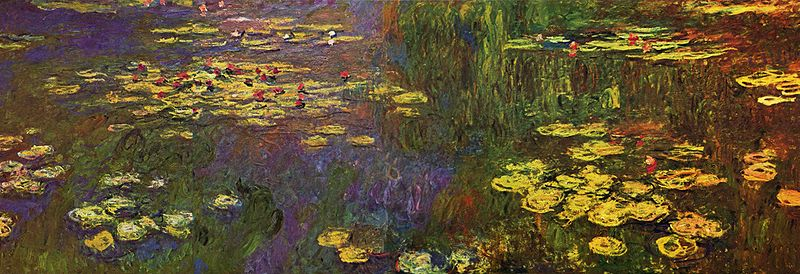
\includegraphics[width=12cm]{800px-Claude_Monet_038.jpg}
          \caption{睡莲(原作属于公有领域,编译版权归Zenodot Verlagsgesellschaft mbH,依GFDL协议使用)}
          \label{fig:water-lilies}
        \end{figure}
        
    \section{逝世}
    \esection{Death}
    
        他于1926年12月5日死于肺癌,享年86岁,下葬于吉维尼教堂的墓地。莫奈坚持葬礼的仪式要简单,因此大约只有五十人出席了他的葬礼。
        
        他的家,他的花园和睡莲由唯一继承人也就是他的儿子米歇尔继承,并于1966年捐赠给法国美术学院。通过莫奈基金会,他的房子和花园在1980年复原后开放参观。除了莫奈的纪念品和他一生中的其他事物,房子中还包含了他收集的日本木刻版画他的房子也是吉维尼两个主要景点之一。

        \begin{figure}[h!]
          \centering
          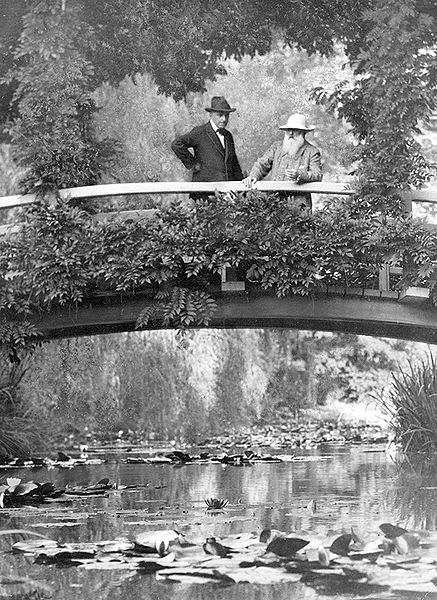
\includegraphics[width=6.67cm]{437px-Monet_in_Garden_New_York_Times_1922.jpg}
          \caption{莫奈在他的花园中。右为莫奈(公有领域)}
          \label{fig:monet-in-gardon}
        \end{figure}

    \section{作品的销售}
    \esection{Posthumous sales}
        
        2004年,莫奈的\textit{the Parliament}和\textit{Effects of Sun in the Fog}在伦敦卖出了超过2000万美元。2006年,英国皇家学报发表文章指出这两幅画作是在泰晤士河上的圣托马斯医院创作的。
    
        他的作品《迪耶普附近的悬崖》被盗两次。一次是在1998年,博物馆的馆长被裁定与两名同伙一起盗窃,因此被判入狱五年零两个月;另一次是在2007年8月,并于2008年找回。他在1873年创作的作品\textit{Le Pont du chemin de fer \`a Argenteuil},描绘了巴黎附近塞纳河上的一座铁路桥。这幅作品2008年5月6日被一个匿名电话竞标者在纽约克里斯蒂拍卖行以4140万美元竞得。在此之前,他的单幅作品售价的最高记录是3650万美元。仅仅几周之后的2008年6月24日,睡莲系列中的\textit{Le bassin aux nymphas}在伦敦佳士得拍出。落锤价是36,500,000英镑\footnote{71,892,376.34美元},算上竞拍费用高达40,921,250英镑\footnote{80,451,178美元},是当时最贵的20幅画作之一。


        % jiang-hk.tex
%
% Aetf <aetf@unlimitedcodeworks.xyz>
% Copyright 2016 Aetf <aetf@unlimitedcodeworks.xyz>
%
% multiple1902 <multiple1902@gmail.com>
% Copyright 2011~2012, multiple1902 (Weisi Dai)
%
% Project Home: https://github.com/Aetf/xjtuthesis
%
% It is strongly recommended that you read documentations located at
%   https://github.com/Aetf/xjtuthesis/wiki
% in advance of your compilation if you have not read them before.
%
% This work may be distributed and/or modified under the
% conditions of the LaTeX Project Public License, either version 1.3
% of this license or (at your option) any later version.
% The latest version of this license is in
%   http://www.latex-project.org/lppl.txt
% and version 1.3 or later is part of all distributions of LaTeX
% version 2005/12/01 or later.
%
% This work has the LPPL maintenance status `maintained'.
%
% The Current Maintainer of this work is Aetf.
%
\chapter{江学长怒斥香港记者}

(2000年10月27日,北京中南海)

港女记:江主席,你觉得董先生连任,好不好啊?

江学长:好喔!

港女记:中央也支持他哈?

江学长:当然啦!

港女记:那为什么这么早就决定了,而不考虑别的人选了?

港女记:欧盟呢,最近发表了一个报告说呢,北京会透过一些渠道去影响、干预香港的法治。你对这个看法有什么回应呢?

江学长:没听到过!

港女记:这是彭定康说的。

江学长:彭定康说的就是真的了?你们媒体千万要注意了,不要见着风是得雨,接到这些消息,媒体本身也要判断,明白这意思吗?假使这些完全无中生有的东西,你再帮他说一遍,你等于……你也有责任吧?

港女记:现在那么早,你们就说支持董先生,会不会给人一种感觉,就是内定呀、是钦点呀董先生呀?

江学长:没有,没有任何的意思!还是按照香港的、按照基本法、按照选举的法,去产生……

港女记:但是你们能不能……

江学长:刚才你们问我呀,我可回答你一句「无可奉告」。但是你们又不高兴,那怎么办?!

港女记:可……

江学长:我讲的意思,不是钦点他当下一任。你问我支持不支持,我说支持。我就明确给你、告诉你。

港女记:江主席……

江学长:但是你们吧,你们……我感觉你们新闻界,还要学习一个……你们非常熟悉西方的那一套的理论,你们毕竟还too young!明白这意思吗?!我告诉你们,我是身经百战了,见得多了。西方的哪个国家我没去过?你们要知道,美国的华莱士,那比你们不知要高到哪里去了!嗯,我跟他谈笑风生。就是说媒体呀,还是要提高自己的知识水平。识得不识得啊?

江学长:唉,我也替你们着急呀,真的。你们就……你们有一个好,全世界跑到什么地方,你们比其他的西方记者,跑得还快!但是问来问去的问题呀,都too simple,sometimes na\"ive。懂了没啊?

港女记:可江主席……哦……

港女记:能不能说一下,为什么要支持董先生?

江学长:我很抱歉,我今天是作为一个长者,跟你们讲的。我不是新闻工作者,但是我见得太多了……我……有这个必要告诉你们一点,人生的经验。

江学长:刚才我很想啊,就我每次碰到你们,我就想到中国有句话叫「闷声发大财」。

港男记:那叫什么话?一句……

江学长:这是最好的!但是我想我见到你们这样热情呀,一句话不说也不好。所以刚才你一定要……在宣传上将来如果你们报道上敢有偏差,你们要负责!我没有说要钦定,没有任何这个意思。但是你问,一定要问我,对董先生支持不支持。我们不支持他?他现在当特首,我们怎么能不支持特首?!对不对?

港女记:但是如果说连任呢?

江学长:哎,连任也按照香港的法律呀,对不对?要、要按着香港的……当然我们的决定权,也是很重要的!香港特区、特别行政区是属于中国、中华人民共和国中央人民政{}府,啊!到那个时候,我们会表态的!

港女记:但是呢……

江学长:明白这个意思吗?你们呀,不要想喜欢,啊,弄那么个大新闻,说现在已经钦定了,就把我批判一番!

问:但是……

江:你们啊,Na\"ive ……I'm angry,我跟你们讲,你们这样子不行的。我今天算得罪了你们一下。


        
\chapter{总结与展望}
\echapter{Conclusions}

从项目的第一行代码写下到修复已知的最后一个bug且将项目暂时尘封,历时7个月。作为笔者本科阶段工作量最大的项目,它的工作并非简单地设计出工程架构、堆砌业务逻辑,还包括阅读理解大量Linux文档和已有开源库的实现。

\section{结论}{}

本文首先使用两步提升法对RGB单目单人视频分别进行了人体姿态序列的二维和三维的估计,并进一步搭建了一个完整的视频动作捕捉制作三维动画的框架。

% todo 可补充

在人体姿态估计任务方面,本文的工作可以对日常的人体姿态进行较为准确的还原,但目前的工作还具有以下局限性:
\begin{enumerate}
    \item 网络的泛化性不足。对快速的动作预测出的姿态速度较慢,对快速运动时不清晰帧的预测效果有限,对于非常见动作的预测准确性较差,在背景复杂时易出现混淆的情况。
    \item 网络对于上下文信息的提取能力有限。当对于多个三维姿态对应相同的二维姿态投影的歧义性发生时,易估计出反人体解剖学的三维姿态。
    \item 模型对于世界坐标系中人体根节点的位移的估计效果较差。
\end{enumerate}

在视频动作捕捉制作三维动画方面,本文的工作可以利用人体的动作制作出生动且还原度高的三维角色动画,但对于原始视频的采集仍具有以下要求:
\begin{enumerate}
    \item 固定相机位姿拍摄单人视频,保证人体部位全部入境。
    \item 目标人物距离与镜头的距离位于3到10米之间。
    \item 人物衣着简单,背景干净,避免遮挡与混淆。
\end{enumerate}

6.2 展望
针对如上问题,针对本文课题的未来工作仍然具有诸多挑战和极大的发展空间,也有诸多值得期待的改进方向:
\begin{enumerate}
    \item 在实际应用场景中,可以相应地丰富数据集,对不同距离,速度的动作进行全方面的采集。
    \item 人体姿态估计虽然具有着许多固有的难点,如投影歧义等。但人体本身的解剖学约束,以及人体动作中包含的丰富的语义信息以及上下文信息可以对姿态的估计提供高强度的帮助。可以利用如图卷积神经网络等模型,对如上深层信息进行进一步的提取。
    \item 视频动作捕捉的市场广阔,针对动作制作需求,可以对提取出的动作序列进行针对性的后处理优化,如消抖、平滑、清洗突变帧,稳定根节点位移,增强脚-地接触的重力效果等。
\end{enumerate}




    \xjtuendcontent

    \xjtubib{sample}

    \xjtuappendix

        % appendice.tex
%
% Aetf <aetf@unlimitedcodeworks.xyz>
% Copyright 2016 Aetf <aetf@unlimitedcodeworks.xyz>
%
% multiple1902 <multiple1902@gmail.com>
% Copyright 2011~2012, multiple1902 (Weisi Dai)
%
% Project Home: https://github.com/Aetf/xjtuthesis
%
% It is strongly recommended that you read documentations located at
%   https://github.com/Aetf/xjtuthesis/wiki
% in advance of your compilation if you have not read them before.
%
% This work may be distributed and/or modified under the
% conditions of the LaTeX Project Public License, either version 1.3
% of this license or (at your option) any later version.
% The latest version of this license is in
%   http://www.latex-project.org/lppl.txt
% and version 1.3 or later is part of all distributions of LaTeX
% version 2005/12/01 or later.
%
% This work has the LPPL maintenance status `maintained'.
%
% The Current Maintainer of this work is Aetf.
%
\xjtuappendixchapter{附录}

    \xjtuappendixsection{测试标题}

        The quick brown fox jumps over the lazy dog.

        \begin{figure}[h!]
          \centering
          
\includegraphics[width=6.67cm]{XJTU.pdf}
          \caption{西安交通大学}
          \label{fig:in-appendix}
        \end{figure}

        \xjtuappendixsubsection{三级标题}

            测试

            \xjtuappendixsubsubsection{四级标题}

                测试

\xjtuappendixchapter{还是附录}

    \xjtuappendixsection{测试}

        The quick brown fox jumps over the lazy dog.


    \xjtuendappendix

    \xjtuspchapter{致谢}{致\qquad 谢}{Acknowledgements}

        美哉吾校, 真理之花, 青年之模楷, 邦国之荣华, 

校旗飘扬, 与日俱长, 为世界之光, 为世界之光. 

美哉吾校, 鼓舞群伦, 启发我睿智, 激励我热忱, 

英俊济跄, 经营四方, 为世界之光, 为世界之光. 

美哉吾校, 性灵泉源, 科学之奥府, 艺术之林园, 

实业扩张, 进步无疆, 为世界之光, 为世界之光. 

美哉吾校, 灿烂文明, 实学培国本, 民族得中兴, 

宇土茫茫, 山高水长, 为世界之光, 为世界之光. 


    \xjtuspchapter{攻读博士期间取得的研究成果}{攻读博士期间取得的研究成果}{Achievements}

        \begin{enumerate}
            \item 已发表或已录用的学术论文、已出版的专著/译著、已获授权的专利按参考文献格式列出。
            \item 科研获奖,列出格式为:\\
                获奖人(排名情况).项目名称.奖项名称及等级,发奖机构,获奖时间.
            \item 与学位论文相关的其它成果参照参考文献格式列出。
            \item 全部研究成果连续编号编排。
        \end{enumerate}

    \xjtuacademicintegrity


\end{document}

